\chapter{Methodology}
\label{chp:method}

In this chapter, we explain the method developed to locate the occupancy sensors in a ceiling mounted sensor grid, using the  data obtained from the sensors and  information about the locations of the vertices of the grid.
Consider a sensor grid as shown in the Figure \ref{fig:Grid}, consisting of n nodes. There are $N= n!$ ways in which these sensors can be uniquely placed on the grid. 
Out of these $N$ ways we have to identify the actual locations of the sensors in the grid.
\begin{figure}[!ht]
\begin{tikzpicture}
%\draw(0+rand,0+rand) node[circle,fill=black]{};
%\draw(1.5+rand,0+rand) node[circle,fill=black]{};

%\draw(0+rand,2+rand) node[circle,fill=black]{};
%\draw(1.5+rand,2+rand) node[circle,fill=black]{};
\draw(0,4) node[circle,fill=black]{};
\draw(1.5,4) node[circle,fill=black]{};
%\foreach \x in {0,1,2,3,4}
 %   \foreach \y in {0,1,2} 
%  {
 %      \node [fill,circle]  (\x\y) at (\x+rand,\y+rand) {};} 
%\draw(4,0) node[circle,fill=black]{};
%\draw(4,2) node[circle,fill=black]{};
%\draw(4,3.5) node[circle,fill=black]{};
\foreach \x in {2,3,4,5,6}
    \foreach \y in {4} 
  {
       \node [fill,circle]  (\x\y) at (\x+0.25*rand,\y+0.25*rand) {};
   } 
   \foreach \x in {0,1,2,3,4,5,6}
    \foreach \y in {0,1,2,3} 
  {
       \node [fill,circle]  (\x\y) at (\x+0.25*rand,\y+0.25*rand) {};
   }
       
       \draw[thick](0,4) circle(1cm);
       \draw[|->|, rotate around with nodes={90:(0,4)}]
       (0,4)--(1,4) node[midway,fill=white,rotate with]{r};
       \draw[|<->|](0,4)--(1.5,4) node[midway,fill=white]{d};
       \draw[thick](1.5,4) circle(1cm);
       
%\draw [decorate,decoration={brace,amplitude=10pt},xshift=-4pt,yshift=0pt]
%(-0.5,0) -- (-0.5,3.5) node [black,midway,xshift=-0.6cm] 
%{\footnotesize $M$};

%\draw [decorate,decoration={brace,mirror,amplitude=10pt},xshift=-1em,yshift=-2em](0,-0.3) -- (4.5,-0.3) node [black,midway,yshift=-0.6cm]{\footnotesize N};


\end{tikzpicture}
\centering
\caption{A sensor grid with sensors field of view being $ r$.}
\label{fig:Grid}
\end{figure}
Before we explain the method, we introduce the definitions of the terms that are used in the thesis.
\begin{definition}{Neighboring sensors:}
 Two sensors are said to be neighbors if they have overlapping field of view.
\label{def:ns}
\end{definition}
\begin{definition}{Grid Adjacency Matrix:}
 We represent the sensor grid in the form of an adjacency matrix. Two vertices of the grid $i$ and $j$ are adjacent if the distance between them ($d_{i,j}$) is less than twice the radius $(r)$ of the sensor's field of view.

\[
GAM_{i,j} = 
\begin{cases}
1, &\text{ if } d_{i,j} < \text{  2r } \forall \text{ } i \ne j\\
0, & \text{otherwise}\\
\end{cases}
    \]
$d_{i,j}$  is the euclidean distance between the vertex $ i(x_i,y_i)$ and $j(x_j,y_j)$.
\begin{equation*}
d_{i,j}=\sqrt{(x_i-x_j)^2 + (y_i-y_j)^2}
\end{equation*}
\label{def:GAM}
\end{definition}
From the definitions \ref{def:ns} and \ref{def:GAM}, we can say that sensors placed on neighboring vertices will be neighboring nodes and vise versa. As can be seen in the Figure \ref{fig:Grid} there will be an overlap in the field of view between two sensors if the distance $(d)$ between them is less than $2r$.

\section{Feature}
\label{sec:energy}
As it has been shown previously in \cite{Hong:2013:TAS:2528282.2528302,doi:10.1061/9780784413616.226,Koc:2014:CLC:2674061.2674075}, that the neighboring sensors can be identified by computing the correlation values for the sensors raw data or a feature extracted from the raw sensor data. We commence our method similarly by identifying a feature which will aid us to do the same. As neighboring sensors have an overlapping field of view, they observe the same events and thus are highly correlated. On the raw signals of the PIR data stream we use a sliding window with $50\%$ overlap between the consecutive windows and compute the energy feature using the equation \ref{eq:energyEq}. 50\% overlapping window has been chosen as it has been shown to be effective for feature extraction previously\cite{bao2004activity}. We determine the window length empirically.
\begin{equation}
\label{eq:energyEq}
E_s = {\sum_{m=0}^{k}{|a[m]|}^2},
\end{equation}
where $a[m]$ - Discrete time signal.

For a PIR sensors whose output is binary, computing energy reduces to counting the number of triggers observed within the window.

With the newly computed energy data stream, we compute the cross correlation between all the sensors using equation \ref{eq:corrcoeff}
\begin{equation}
\label{eq:corrcoeff}
r_{X,Y}=\frac{\sum_{i=1}^{m}(X_i-\overline{X})(Y_i-\overline{Y})}{\sqrt{\sum_{i=1}^{m}(X_i-\overline{X})^2}\sqrt{\sum_{i=1}^{m}(Y_i-\overline{Y})^2}} \\
\end{equation}
where $X$ and $Y$ are data streams.\\
 $X_i$ and $Y_i$ are the $i^{\mbox{th}}$ sample of the data stream $X$ and $Y$, respectively.\\
$\overline{X}$ and $\overline{Y}$ is the mean value of $X$ and $Y$ respectively.\\
 $m$ is the number of samples.


\section{Grid Correlation Sum}
\label{sec:gcs}
Using the cross correlation values between the sensors, we define correlation matrix $R$ between the $n$ sensor nodes as shown in the equation \ref{eq:corrMatrix}. The matrix $R$ is constructed such that $R(i,j)$ corresponds to the correlation value between the sensors $i$ and $j$.
\begin{equation}
\label{eq:corrMatrix}
\centering
R = 
\begin{bmatrix}
    r_{1,1} & r_{1,2} & \dots  & r_{1,n} \\
    r_{2,1} & r_{2,2}  & \dots  & r_{2,n} \\
    \vdots & \vdots  & \ddots & \vdots \\
    r_{n,1} & r_{n,2}  & \dots  & r_{n,n}
\end{bmatrix}
\end{equation}\\
$r_{\alpha,\beta}$ represents correlation value between the energy stream for sensor $\alpha$ and $\beta$.\\


Using \textit{correlation matrix} ($R$) and \textit{Grid Adjacency Matrix} $(GAM)$ we define a quantity called \textit{Grid Correlation Sum (GCS)} as given in the equation \ref{eq:gridCorrelationSum}. $GCS$ represents the sum of correlation value of the sensor pair residing on neighboring vertices of the grid.
As the matrices are symmetrical along the diagonals we only consider the elements of the upper triangle of the matrices excluding the diagonal elements. 

\begin{equation}
\centering
GCS=\sum_{i=1}^{n-1}\sum_{j=i+1}^{n} R(\phi(i),\phi(j))  \times GAM(i,j)
\label{eq:gridCorrelationSum}
\end{equation}
$i,j$ represent $ i^{th}$ and $ j^{th}$ vertex on the grid.\\
$\phi$ is a mapping functions which gives the sensor located at vertex $i$.\\
$ R(\phi(i),\phi(j))$: correlation coefficient between the sensors placed on vertex $i$ and $j$.\\
$GAM$:  Adjacency matrix of the grid as per definition \ref{def:GAM}.\\

We use $GCS$ to identify the correct arrangement out of all the $N$ possible arrangements. We hypothesize that if we compute $GCS$ for all the possible arrangements, the arrangement with the maximum $GCS$ will represent the actual arrangement of the sensors on the grid. The reasoning behind the hypothesis is that, if two non-neighboring sensors are kept on neighboring vertices or vice versa then the correlation value between those two sensors will be low and thus decreasing the $GCS$.
To illustrate this consider a sensor grid as shown in the Figure \ref{fig:arrangement1}.
 It consists of 3 $\times$ 3 grid.  
$GCS$ for the grid is :\\
\begin{equation*}
GCS_{1}=\text{r(1,2)+ r(1,4)+...\textbf{r(2,3)}+...\textbf{r(5,6)}+\textbf{r(6,9)}..+r(8,9)}
\end{equation*}

Now consider the arrangement shown in Figure \ref{fig:arrangement2}, where the position of the sensors 3 and 6 are interchanged\\
\begin{equation*}
GCS_{2}=\text{ r(1,2)+r(1,4)+...+\textbf{r(2,6)}+...+\textbf{r(3,5)+r(3,9)}...+r(8,9)}
\end{equation*}

\begin{figure}[!ht]
\begin{floatrow}
\ffigbox{
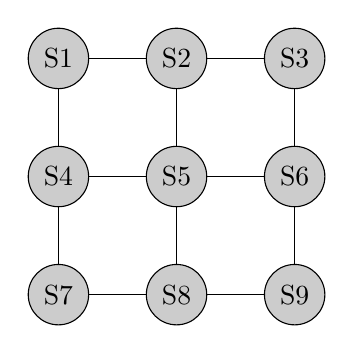
\begin{tikzpicture}[darkstyle/.style={circle,draw,fill=gray!40,minimum size=5}]
\foreach \y in {0,1,2}
 \foreach \x in {0,1,2}
{\pgfmathtruncatemacro{\label}{\x-3*\y+7}
\node[darkstyle](\x\y) at (1.5*\x,1.5*\y){S\label};
}
 \foreach \x in {0,1,2}
    \foreach \y [count=\yi] in {0,1}  
      \draw (\x\y)--(\x\yi) (\y\x)--(\yi\x) ;

\end{tikzpicture}

\caption{Actual arrangement of sensors on the grid.}
\label{fig:arrangement1}
}

\ffigbox{
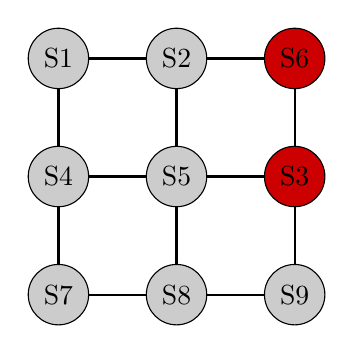
\begin{tikzpicture}[darkstyle/.style={circle,draw,fill=gray!40,minimum size=5}]

\draw[step = 1.5,thick ] (7.4,0) grid (10.5,3);
\node[circle,draw=black,fill=white!80!black,minimum size=5] (7) at (7.5,0) {S7};
\node[circle,draw=black,fill=white!80!black,minimum size=5] (4) at (7.5,1.5) {S4};
\node[circle,draw=black,fill=white!80!black,minimum size=5] (1) at (7.5,3) {S1};

\node[circle,draw=black,fill=white!80!black,minimum size=5] (8) at (9,0) {S8};
\node[circle,draw=black,fill=white!80!black,minimum size=5] (5) at (9,1.5) {S5};
\node[circle,draw=black,fill=white!80!black,minimum size=5] (2) at (9,3) {S2};

\node[circle,draw=black,fill=white!80!black,minimum size=5] (9) at (10.5,0) {S9};
\node[circle,draw=black,fill=red!80!black,minimum size=5] (3) at (10.5,1.5) {S3};
\node[circle,draw=black,fill=red!80!black,minimum size=5] (6) at (10.5,3) {S6};
%\draw [<->,red] (3.east) to [out=60,in=60] (6.east);

\end{tikzpicture}

\caption{Incorrect arrangement of sensors on the grid.}
\label{fig:arrangement2}
}
\centering

\end{floatrow}
\end{figure}

$GCS_{1}$ will be greater than $GCS_{2}$ as $r(2,3)>r(2,6)$ , $r(5,6) > r(3,5)$ and $ r(6,9) > r(3,9)$ as sensor pair [2,6] , [3,5] and [3,9] are non-neighboring sensor nodes placed on neighboring vertices. Hence we can say that $GCS$ will be maximum for a  mapping which maps sensors onto the grid accurately.\\
With this condition, a straightforward way to determine the sensor location will be to carry out a brute force search where $GCS$ is computed for all the $N$ possible arrangements. The brute force search can be carried out only when the number of sensors is low, as the number of sensors increases the number of possible mappings also increase drastically, which makes it impossible to carry out a brute force search. Hence there is a need to reduce the search space.


\section{Maximum spanning Tree}

Having established a criterion to determine the right arrangement of sensors on the grid from  possible ${N}$ arrangements. The next step is to reduce the search space.

According to definitions [\ref{def:ns}, \ref{def:GAM}], in a sensor grid if one of the sensors are placed on a grid vertex then the neighboring vertex has to be occupied by a neighboring sensor. Consider a sensor grid as shown in the Figure \ref{fig:prune}, sensor $S_1$ is mapped to one of the vertex of the grid, vertices $a,b,c,\text{ and }d$ are its neighboring vertices. Now sensor $S_2$, which is a neighboring sensor of $S_1$ can only occupy one of the vertices among $a,b,c\text{ or }d$. If this condition was not employed then $S_2$ could have occupied any of the unoccupied vertices on the grid and thus increasing the search space. If we are able to identify a neighboring sensor for a sensor node, we can reduce the search space by eliminating the arrangements which place a non-neighboring sensor node onto a neighboring vertex or vice versa.
\begin{figure}[!ht]
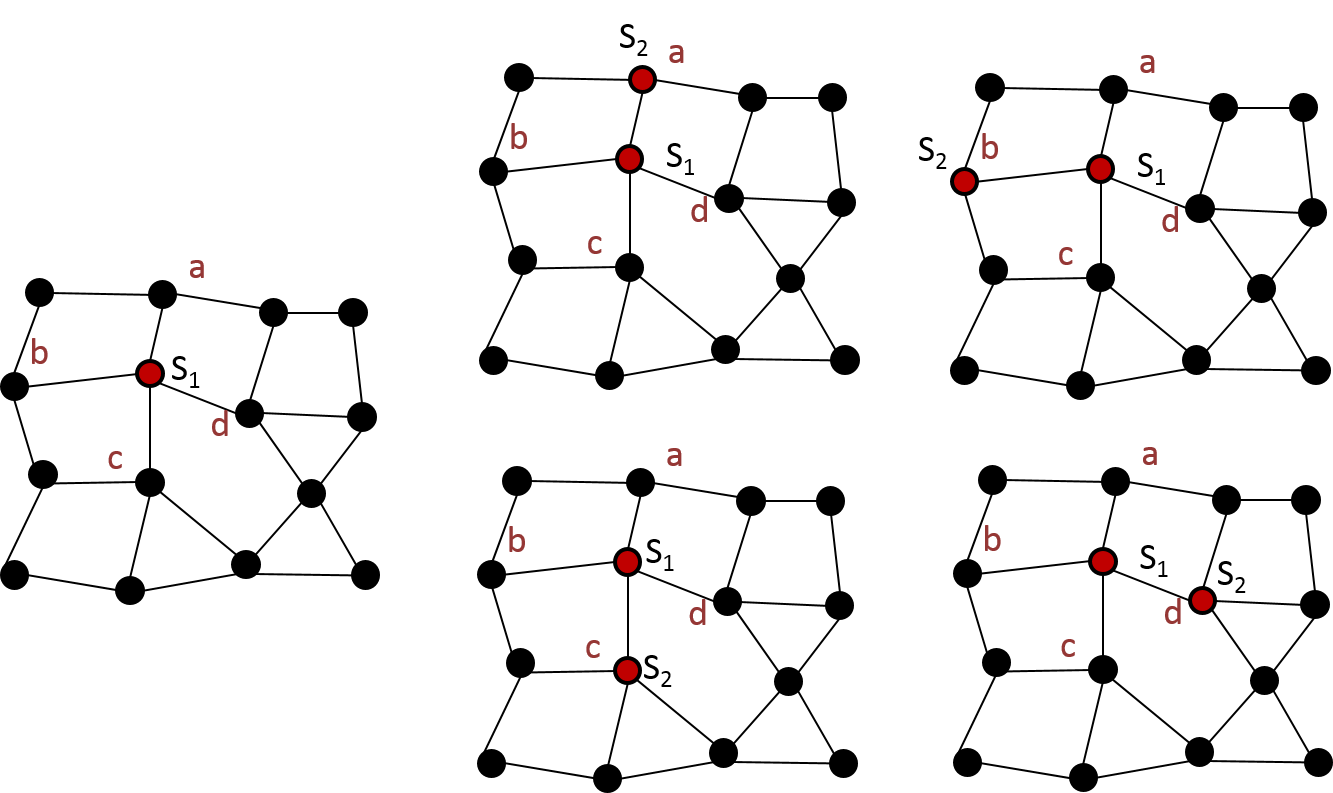
\includegraphics[scale=0.5]{./pics/prune}
\centering
\caption{Possible arrangements of a sensor node when its neighboring node is already mapped on the grid}
\label{fig:prune}
\end{figure}



To identify neighboring sensors, we build a graph $G(V,E,W)$ such that $V = \{S_1,S_2,S_3...S_n\}$ , $ E= \{(S_1,S_2),(S_1,S_3)....(S_{n-1},S_n)\}$, $W = R$ and compute the Maximum Spanning Tree $(MST)$ for it. The generated $MST$ consists of all the sensor nodes connected to at least one other node by an edge. The $MST$ chooses an edge for every sensor such that the weight of the edge outgoing from the sensor $\alpha$ to sensor $\beta$ is the maximum among all the edges starting from sensor $\alpha$, in graph ${G}$. As the weights represent correlation values it implies that the maximum spanning tree connects a node to another with which it has the maximum correlation. As the correlation between the neighboring nodes is maximum we can say that MST connects the neighboring sensors.

To compute MST we make use of Prim's algorithm\cite{BLTJ:BLTJ1515}.  Prim's algorithm is originally used to compute the minimum spanning tree. To compute the maximum spanning tree the weights of the graph $G$ are negated and with these weights, minimum spanning tree is computed using Prim's algorithm. The minimum spanning tree thus obtained represents the maximum spanning tree for the original graph $G$.

As per the definition of $G(V,E,W)$, there is an edge between the neighboring vertices of the grid. The $MST$ as we discussed above is formed by connecting neighboring sensors. Thus we can infer that the $MST$ over $R$ represents a spanning tree for the graph $G$. 

\begin{figure}[!ht]
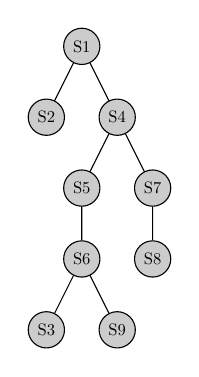
\begin{tikzpicture}[scale=0.6,darkstyle/.style={circle,draw,fill=gray!40,minimum size=5,transform shape}]
\node[darkstyle]{S1}
    child{node[darkstyle]{S2}}
    child{node[darkstyle]{S4}
        child{node[darkstyle]{S5}
            child{node[darkstyle]{S6}
                child{node[darkstyle]{S3}}
                child{node[darkstyle]{S9}}}}
                child{node[darkstyle]{S7}
                child{node[darkstyle]{S8}}}};
\end{tikzpicture}
\qquad \qquad \qquad
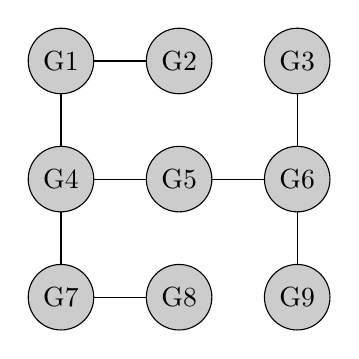
\begin{tikzpicture}[darkstyle/.style={circle,draw,fill=gray!40,minimum size=3}]
\foreach \y in {0,1,2}
 \foreach \x in {0,1,2}
{\pgfmathtruncatemacro{\label}{\x-3*\y+7}
\node[darkstyle](\x\y) at (1.5*\x,1.5*\y){G\label};
}
\draw (01)--(02) (02)--(12) (01)--(11) (11)--(21) (21)--(22)
(21)--(20) (00)--(01) (00)--(10);


\end{tikzpicture}
\caption{A maximum spanning tree incident on the grid}
\label{fig:MST}
\end{figure}




It is possible that for a given grid there may be several spanning trees with the same structure. 
Figure \ref{fig:variousMappings} shows few of the spanning tree of the grid similar to the MST obtained for the correlation matrix.
\begin{figure}[!ht]

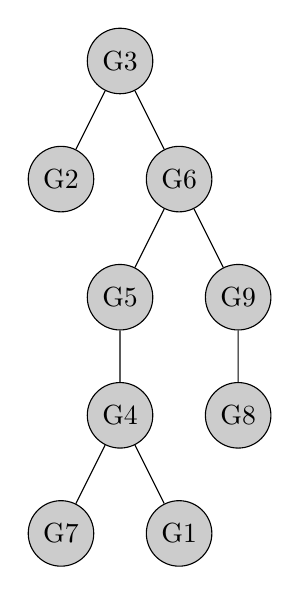
\begin{tikzpicture}[darkstyle/.style={circle,draw,fill=gray!40,minimum size=5}]
\node[darkstyle]{G3}
    child{node[darkstyle]{G2}}
    child{node[darkstyle]{G6}
        child{node[darkstyle]{G5}
            child{node[darkstyle]{G4}
                child{node[darkstyle]{G7}}
                child{node[darkstyle]{G1}}}}
                child{node[darkstyle]{G9}
                child{node[darkstyle]{G8}}}};
\end{tikzpicture}
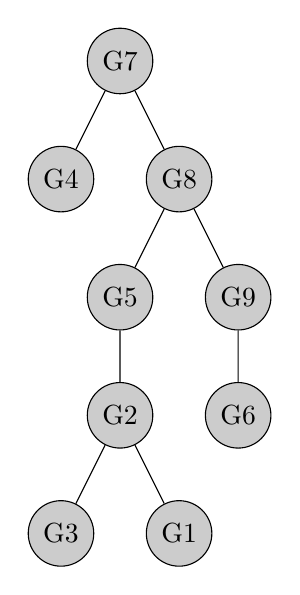
\begin{tikzpicture}[darkstyle/.style={circle,draw,fill=gray!40,minimum size=5}]
\node[darkstyle]{G7}
    child{node[darkstyle]{G4}}
    child{node[darkstyle]{G8}
        child{node[darkstyle]{G5}
            child{node[darkstyle]{G2}
                child{node[darkstyle]{G3}}
                child{node[darkstyle]{G1}}}}
                child{node[darkstyle]{G9}
                child{node[darkstyle]{G6}}}};
\end{tikzpicture}
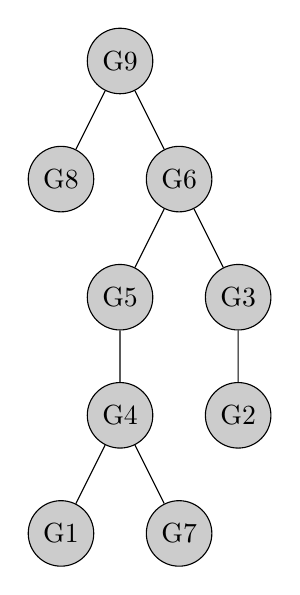
\begin{tikzpicture}[darkstyle/.style={circle,draw,fill=gray!40,minimum size=5}]
\node[darkstyle]{G9}
    child{node[darkstyle]{G8}}
    child{node[darkstyle]{G6}
        child{node[darkstyle]{G5}
            child{node[darkstyle]{G4}
                child{node[darkstyle]{G1}}
                child{node[darkstyle]{G7}}}}
                child{node[darkstyle]{G3}
                child{node[darkstyle]{G2}}}};
\end{tikzpicture}
\caption{Various spanning tree for the grid with similar structure of the MST of the correlation matrix.}
\label{fig:variousMappings}
\end{figure}


If we compute all the possible spanning trees for the grid which maintains the same structure as that of the $MST$ for the correlation matrix and map each vertex on the MST to the corresponding spanning tree of the grid as shown in the Figure \ref{fig:mapping}, we obtain several possible mappings of the sensors to grid location. Among the possible mappings, we have to choose the correct arrangement. To choose the true arrangement of the sensor on the grid we make use of $GCS$. 
The number of arrangements that are obtained from this method is lesser than the ${N}$  possible arrangements that had to be evaluated for brute force technique.

%The main reason for the decrease in the possible mapping is because when we are computing various mappings between the sensors maximum spanning tree and spanning tree for the grid, adjacency has to be maintained. Which implies that when sensor $S_1$ gets assigned to grid vertex $G_1$, while assigning sensor $S_2$ which is a neighbor of $S_1$ to the grid vertices, care has to be taken that the assigned grid node has to be a neighbor of the vertex $G_1$.









%Having established a method to determine the true arrangement of the sensor nodes on the grid from all the possible \textbf{N} arrangements, the next step is to prune the possible arrangements. \\
%From the definitions of neighboring sensors and neighboring vertices we can say that two neighboring sensors will always be placed on the neighboring vertices. From the grid adjacency matrix, we can determine the neighboring vertices of a vertex. If we can determine the neighboring sensor nodes then we can prune the number of possible arrangements by using the constraints that only neighboring sensors can occupy the neighboring vertices. 




%If the neighbors of a sensor are known , the sensors occupying the neighboring vertices on the grid has to be occupied by its neighboring sensors .
%The neighboring vertices of a vertex \textbf{i} on which a sensor \textbf{a} is located should be occupied by the neighbors of sensor \textbf{a}.
%Thus resulting in the reduction of the number of possible arrangements.

%If we know which are all the neighbors of a sensor then when a sensor is placed on the vertex of a sensor, we know that the neighboring vertex on the grid should only be occupied by its neighboring nodes. 

%Though the correlation value between two neighboring nodes are high compared to the correlation value between the non-neighboring nodes, finding a threshold to differentiate between the neighboring and non-neighboring nodes when the arrangement is not known is nontrivial.\\
%Although we might not be able to identify all the neighboring nodes even if we are able to find a minimum of one neighboring node per node we will be able to reduce the number of mappings that needs to be checked. To achieve this we calculate the maximum spanning tree for the correlation matrix \textbf{R}.

%If we consider R as an adjacency matrix with each sensor representing a vertex and the correlation value between the sensors representing the edge weight between them. Then the maximum spanning tree for such a graph will connect all the vertices together such that the total weight for the edges in the tree is maximum. 


%A maximum spanning tree has an edge between 2 nodes which have high correlation matrix compared with the other nodes. Therefore if an edge exists between two nodes in the maximum spanning tree then we can say that those two nodes are neighboring nodes.\\
%To compute the maximum spanning tree we use Prim's algorithm \cite{BLTJ:BLTJ1515}.Originally  Prim's algorithm is designed to compute the minimum spanning tree for a graph. In order to compute the maximum spanning tree, the correlation matrix is negated and given as the input to the algorithm. The minimum spanning tree %obtained from negated weights is the maximum spanning tree for the original weights.This maximum spanning tree represents one of the spanning trees for the grid as can be seen from the figure \ref{fig:MST}. 

%A Maximum spanning tree chooses an edge which has the maximum weight starting from the vertex, among all the vertices that are present. As in our case, the vertices represent the sensor nodes and edge weights is the correlation value between the sensor nodes. So  edge that is originates from the node connects to a node which is its neighbor . As this step is carried on for every sensor , we have an edge originating from the sensor node, let's call it  the start node terminating at another sensor node, let's call it end node. The start node has the highest correlation with the end node. As the correlation values who are neighbors are the highest, we can safely tell %that this edge is connecting the start node to a neighbor of the start node.

%While computing the maximum spanning tree an edge from a node under consideration is chosen which has the maximum weight originating from it. out of all the edges, the node has, the edge with the maximum weight is chosen. 

%While computing a maximum spanning tree an edge from a node is chosen which has the maximum weight compared to the other edges of the node under consideration. This process is repeated for all the nodes that are present in the graph. In our case, each vertex represents a sensor and the edge weight is given by the cross %correlation value between the two sensors. Since for every node, a maximum correlation value is chosen and as the correlation value between the neighbors is maximum we can say that in a maximum spanning tree two  neighboring sensors are connected. 










\begin{figure}[!ht]
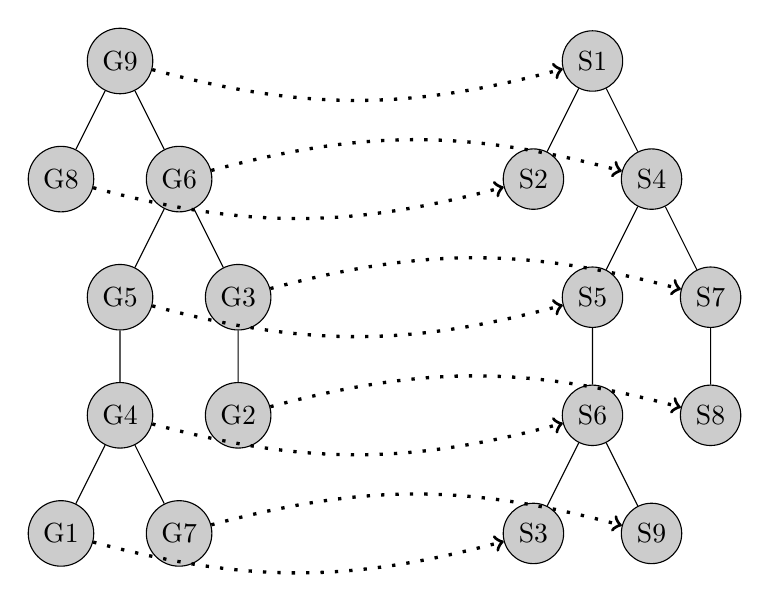
\begin{tikzpicture}[darkstyle/.style={circle,draw,fill=gray!40,minimum size=5}]
\begin{scope}
\node[darkstyle](G9){G9}
    child{node[darkstyle](G8){G8}}
    child{node[darkstyle](G6){G6}
        child{node[darkstyle](G5){G5}
            child{node[darkstyle](G4){G4}
                child{node[darkstyle](G1){G1}}
                child{node[darkstyle](G7){G7}}}}
                child{node[darkstyle](G3){G3}
                child{node[darkstyle](G2){G2}}}};
\end{scope}
\qquad
\begin{scope}[shift={(6,0)}]
\node[darkstyle](S1){S1}
    child{node[darkstyle](S2){S2}}
    child{node[darkstyle](S4){S4}
        child{node[darkstyle](S5){S5}
            child{node[darkstyle](S6){S6}
                child{node[darkstyle](S3){S3}}
                child{node[darkstyle](S9){S9}}}}
                child{node[darkstyle](S7){S7}
                child{node[darkstyle](S8){S8}}}};
\end{scope}
\draw[loosely dotted,very thick,->] (G9)to[out=0-15,in=195](S1);
\draw[loosely dotted,very thick,->] (G8)to[out=0-15,in=195](S2);
\draw[loosely dotted,very thick,->] (G6)to[out=15,in=165](S4);
\draw[loosely dotted,very thick,->] (G5)to[out=0-15,in=195](S5);
\draw[loosely dotted,very thick,->] (G4)to[out=0-15,in=195](S6);
\draw[loosely dotted,very thick,->] (G1)to[out=0-15,in=195](S3);
\draw[loosely dotted,very thick,->] (G7)to[out=15,in=165](S9);
\draw[loosely dotted,very thick,->] (G3)to[out=15,in=165](S7);
\draw[loosely dotted,very thick,->] (G2)to[out=15,in=165](S8);
\end{tikzpicture}
\caption{Mapping between the grid spanning tree and the MST for the correlation matrix}
\label{fig:mapping}
\end{figure}

% Graph monomorphism 

\section{Graph Matching} 

In the previous section, we obtain a maximum spanning tree from $R$ and saw how this represents a spanning tree for the grid. In addition, we observe that there can be multiple spanning trees whose structure is similar to the $MST$. In this section, we describe a method to obtain all the possible spanning trees that have the same structure as the MST obtained from the correlation matrix of the sensors.
The task of checking if a pattern graph $H$ is contained in a base graph $G$ and obtaining all the mappings from $G$ to $H$ is a standard problem of graph matching.

A graph matching process between two graphs $G$ = $(V_G,E_G)$ and H = $(V_H,E_H)$ consists of determining a mapping M which associates nodes of the graph $G$ to $H$ and vice versa. Different constraints can be imposed onto M which results in different mapping types: monomorphism, isomorphism, graph-subgraph isomorphism are the most popular ones \cite{cordella1999performance}. Our problem falls under the category of graph monomorphism. 

Two graphs 
 $G =( V_G, E_G)$ and
 H =$( V_H, E_H)$  are \textit{monomorphic}  if and only if there exists an injective (node)
mapping $\phi (V_G) \rightarrow  V_H$ : for which $\forall v,w \in V_G:(v,w) \in E_G \Rightarrow (\phi((v),\space \phi(w)) \in E_H.$ \cite{singler2005graph}.

Monomorphism is often confused with subgraph isomorphism. Monomorphism is a weaker kind of subgraph isomorphism.

Two graphs  $G =( V_G, E_G)$ and
 H =$( V_H, E_H)$  are \textit{sub graph isomorphic}  if and only if there exists an injective (node)
mapping $\phi( V_G) \rightarrow  V_H$ : for which $\forall \text{ v,w} \in V_G:(v,w) \in E_G \Leftrightarrow (\phi((v),\space \phi(w)) \in E_H.$ \cite{singler2005graph}.

The relationship between edges of the graphs are equivalence for subgraph isomorphism, and for Monomorphism  relationship  is an implication.

A problem of finding all the Monomorphisms of the pattern graph into the base graph is defined as Monomorphism problem. Graph Monomorphism is an NP-Complete problem \cite{Garey:1979:CIG:578533}.  In section \ref{sec:graphLitReview}, we present related works in the field of graph matching. In our work, we use the VF2 algorithm to obtain the mappings between the spanning tree and grid graph.

\subsection{VF2}

In this section, we give a brief description of the VF2 algorithm.

\begin{figure}

\begin{algorithm}[H]
\begin{algorithmic}
 \LState  \textbf{Procedure} Match(s)\\
\textbf{INPUT:}  an intermediate state s; the initial state $s_0$ has $M(s_0)=\emptyset$\\
\textbf{OUTPUT:} the mappings between two graphs\\
\textbf{Match(s)}\\
 \textbf{IF} M(s) covers all the nodes of $G_2$ \textbf{THEN}\\
\quad \textbf{OUTPUT} M(s)\\
\textbf{ELSE}\\
 \quad    Compute the set P(s) of the pairs of candidates for inclusion in M(s)\\
\quad\textbf{FOREACH} (u,v) $\in$ P(s)\\
\quad\quad\textbf{IF} F(s,u,v) \textbf{THEN}\\
\quad\quad\quad    Compute the state s' obtained by adding (u,v) to M(s)\\
\quad\quad\quad\textbf{CALL} Match(s')\\
\quad\quad\textbf{ENDIF}\\
\quad\textbf{ENDFOREACH}\\
\quad Restore data structure\\
\textbf{ENDIF}\\

\end{algorithmic}
\end{algorithm}
\caption{Pseudo code for VF2 algorithm\cite{cordella2001improved}}
\label{fig:VF2}
\end{figure}


% VF2 explanation 
The VF2 algorithm is a graph matching algorithm to solve graph isomorphism, monomorphism, and  subgraph isomorphism problem. VF2 uses depth-first search method to iterate through all the nodes and recursive backtracking technique to check for all the possible mappings. A process of matching 
a base graph $G$ to a pattern graph $H$ consists of determining a mapping $M$ which associate nodes of the base graph $(G)$ with nodes of the pattern graph $(H)$ and vice versa, with some constraints.
Mapping is expressed as a set of pairs of node $(u,v)$ with $u \in G$ and $v \in H$. 
In VF2 algorithm the process of finding the mapping function is described by a  State Space Representation (SSR). Each state s of the matching process can be associated with a partial mapping solution $M(s)$,
which contains only a subset of $M$. A transition from current state $(s)$ to the next state $(s')$ represents the addition of a mapping $(u,v)$ to the state $s$.

VF2 algorithm introduces a set of rules which helps to prune the number of possible SSR that needs to be checked before obtaining a valid mapping. Figure \ref{fig:VF2} gives a high-level description of the VF2 algorithm. There are 3 important functionalities in the algorithm: 
\begin{itemize}
\item generation of possible mappings $(P(s))$
\item checking of the validity of the mapping $(F(s,u,v))$
\item Restore data structure
\end{itemize}


%Data graph (G), Querry graph(Q)

\subsection{Computation of candidate pair set $P(s)$}
This section explains the method to compute the candidate pair set $P(S)$ for an undirected graph $G$ and $H$. 
For every intermediate state s the algorithm computes $P(s)$, a set of possible mapping pairs. For each pair $p$ belonging to $P(s)$ the feasibility of its addition $F(s,u,v)$ is checked : if the check is successful the next state $s' = s \cup p$ and the whole process recursively applies to $s'$.

To compute $P(S)$ set $T_1(s)$ and $T_2(s)$ are defined for Graph $G$ and $H$ respectively. $T_1$ and $T_2$ are the set of  nodes in $G$ and $H$, which are neighbors of the set of nodes included in the partial mapping state $M(s)$ but are not included in $M(s)$.
Set $P(s)$ will be made of all the node pairs $(u,v)$ with $u$ being a node in $T_1$ with the smallest label  and v being a node in $T_2$ . If  $T_1$ and $T_2$ sets are empty then the set $P(s)$ be calculated by using the sets of nodes not contained in either $G(s)$, $H(s)$.

\subsection{Feasibility Rules}
Feasibility Rules are used to check the consistency of the partial solution $s'$ obtained by adding nodes $u,v$ and prune the search tree. The functionality of the rules is as explained below.

In the algorithm, those candidates $(u,v)$ are pruned if for every neighbor $u'$ of $u$ in the partial mapping, the corresponding node $v'$ is a neighbor of $v$, and vice versa.

The algorithm also compares the number of neighboring nodes of each $u$ and $v$ that are connected to nodes in $M(s)$ but are not
included in $M(s)$. The number of such nodes in the base graph must be greater than or equal to the number of such nodes in the pattern graph.

Finally, the number of neighboring nodes of each of $u$ and $v$ that are not directly connected to nodes in $M(s)$ are compared. The number of 
such nodes in the base graph must be greater than or equal to the number of such nodes in the pattern graph.

\subsection{Restore data structure}
In VF2 algorithm all the vectors that are used to store data have the following property: If an element is assigned a value in a state $s$, it will remain assigned in all states descending from $s$. This property, together with the depth-first strategy of the search is used to avoid the need to store a different copy of the vectors for each state. When the algorithm backtracks, it restores the previous value of the vectors. This was the improvement introduced in the VF2 algorithm. This is illustrated in the Figure \ref{fig:memManagement}. Consider every block to hold the mappings between the base graph and the pattern graph. As can be seen from the figure as one goes down in the tree, a new variable is created for every level, but with restore data structure the same variable is used at every level. When the algorithm has finished traversing all the levels of the search tree, the algorithm without restore data structure will have $N$ variables, whereas one with restore data structure will have only one variable created. Thus reducing the space complexity of the VF2 algorithm to $O(N)$ from $O(N^2)$, which was the case in the VF algorithm.

\begin{figure}[!ht]
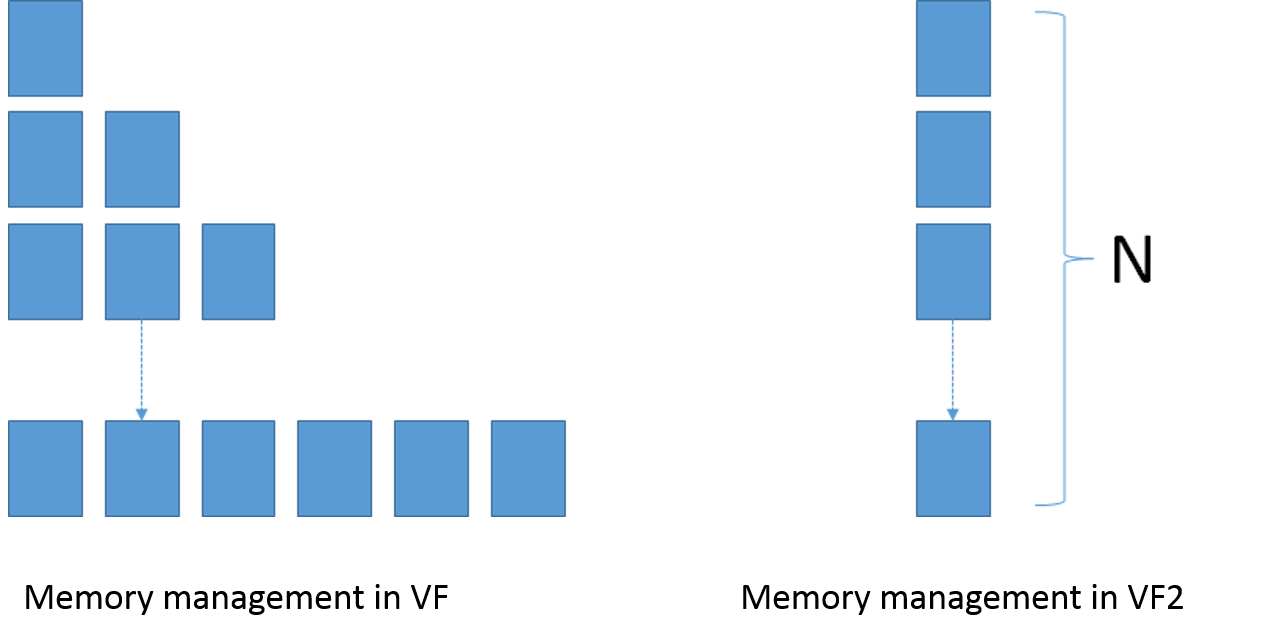
\includegraphics[scale=0.5]{./pics/memManagement.png}
\caption{Memory cells occupied at each state without and with restore data}
\label{fig:memManagement}
\centering
\end{figure}

\subsection{Computation Complexity}
Computational complexity of the VF2 depends on two factors: 
\begin{itemize}
\item The time required to calculate the feasibility of every SSR's , computation of the node pair mappings.
\item Number of SSR visited.
\end{itemize}

According to the \citeauthor{cordella2001improved}, the former has a computational complexity of $O(N)$. For the latter the authors consider a best case; where only one of the potential mappings are feasible which makes the computation complexity $O(N)$ and thus making the overall complexity $O(N^2)$. In the worst case, the algorithm has to explore all the states. This can happen when every node is connected to every other node ( the base graph is a complete graph) and the graph exhibits strong symmetry. The authors show that the complexity in such a condition is $O(N!)$ and thus making the total complexity $O(N!N)$.

The authors compute the computation complexity in the case of an average graph as the reduction in the visited states compared to that of the worst case condition. This reduction is computed using a parameter called $\eta$ which represents the probability of an edge being present between 2 distinct nodes of the graph. The authors show that the average reduction in the number of states visited is:
\begin{equation*}
R_{f}(N) = \prod_{i=1}^{N} 1-(1-\eta)^{i}
\end{equation*}

 
 Variation of $R_f$ for different values of $\eta$ and the number of nodes are as shown in the Figure \ref{fig:compl}. As can be seen in the Figure $R_f$ value converges to a constant as $N$ increases depending on the value of $\eta$. It can also be noticed that as $\eta$ decreases the number of states visited for the same value of $N$ also decreases.
 
 \begin{figure}[!ht]
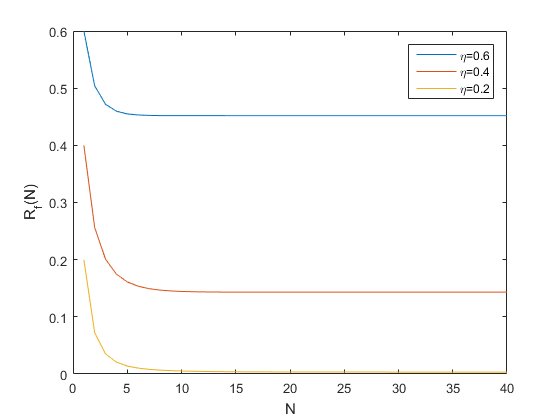
\includegraphics[scale=0.75]{./pics/computation_complexity.png}
\caption{Variation of $R_f$ with $\eta$ and number of nodes N \cite{cordella1999performance}}
\label{fig:compl}
\end{figure}

%In our case, we show the order of complexity for an 8-neighbor grid as shown in the figure \ref{fig:neighborhoodGrid}, we consider such an arrangement as it represents high connectivity that is possible for a sensor grid.
%The worst case for such a grid will arise when at every stage of the search tree the algorithm has to explore every possible branch.
% Since it's an 8-neighborhood grid all the nodes except the ones at the edges of the grid will have 8 neighbors.
% Consider the case as shown in the figure \ref{fig:neighborhoodGrid} for node b it has 7 possible branches (marked in red) other than the branch connected to b, as b is the parent node and has already been assigned.
% As one of the neighboring nodes would be the parent node the node at stage $i$ will have $7^{i}$ possibilities to explore and stage $N$ there will be $7^n$ possibilities to explore as illustrated in the figure \ref{fig:ccO}.
% The total number of states to explore will be given by the sum:
%\begin{flalign*}
%&1 + 7 + 7^2+ . . . . .+7^i+....7^n\\
%&\text{This represents a geometric progression with a= 1, r =7.}\\
%&\text{Sum of a geometric progression is given by:}\\
%&S_{n}=\frac{a(r^n-1)}{r-1}\\
%&S_{n}=\frac{7^{n+1} -1}{7-1} \\
%&\text{When $n$ is large}\\
%&S_{n} \approx 7^N\\
%\end{flalign*}
%
%Thus computational complexity is $O(7^NN)$

%\begin{figure}
%\begin{tikzpicture}
%\draw(0,0) node[circle,fill=black](a){};
%\draw(1,0) node[circle,fill=black](b){};
%\draw(0,1) node[circle,fill=black](c){};
%\draw(1,1) node[circle,fill=black](d){};
%\draw(0,2) node[circle,fill=black](e){};
%\draw(1,2) node[circle,fill=black](f){};
%\draw(0,3) node[circle,fill=black](g){};
%\draw(1,3) node[circle,fill=black](h){};
%
%\draw(2,0) node[circle,fill=black](i){};
%\draw(3,0) node[circle,fill=black](j){};
%\draw(2,1) node[circle,fill=black](k){};
%\draw(3,1) node[circle,fill=black](l){};
%\draw(2,2) node[circle,fill=black,label=above:b](m){};
%\draw(3,2) node[circle,fill=black](n){};
%\draw(2,3) node[circle,fill=black,label=above:a](o){};
%\draw(3,3) node[circle,fill=black](p){};
%\draw[dashed](a)--(b) (b)--(c) (c)--(d) (a)--(d) (b)--(d)
%(e)--(f) (a)--(c) (g)--(h)  (c)--(e) (e)--(g) (h)--(f) 
%(f)--(d) (c)--(f) (e)--(h) (g)--(f)
%
% (i)--(j) (j)--(k)  (k)--(m) (m)--(l) (e)--(i) (i)--(k)(l)--(j) (k)--(m) (n)--(l) 
% (k)--(l)  (m)--(n) (n)--(o) (o)--(p) (i)--(l) (m)--(p) (m)--(o) (m)--(p) (m)--(o)  (m)--(n)
% (p)--(n) (n)--(k)
%(m)--(f) 
% (b)--(i)  (b)--(k)  (d)--(i)  (d)--(m) (f)--(k) (h)--(m) (f)--(o) (d)--(k) (f)--(m) (h)--(o); 
% \draw[red] (m)--(f)  (k)--(m)(m)--(l)  (m)--(p) (m)--(n) (m)--(d) (m)--(h);
% \draw[blue](m)--(o);
%\end{tikzpicture}
%\caption{A 8 neighbor grid}
%\label{fig:neighborhoodGrid}
%\end{figure}
%
%
%\begin{figure}[!ht]
%\includegraphics[scale=0.5]{./pics/tree.png}
%\caption{All the visited states in case of a 8 neighborhood grid with n nodes.}
%\label{fig:ccO}
%
%\end{figure}

\section{Determination of sensor placement}
\label{ref:rotationalSym}
After we obtain the various mappings. We need to decide which out of the various mappings gives the actual placement of the sensors on the grid. To identify the correct mapping we compute $GCS$ as explained in section \ref{sec:gcs}. We calculate the grid correlation sum for all the mappings obtained and the mappings which give the maximum sum will be the actual placement of the sensors on the grid. 
\subsection{Limitations}

Our method  can identify the location of the sensors up to rotational symmetry. A graph is said to posses rotationally symmetry if there exists a point so that the object when rotated a certain number of degrees (or radians) about said point, looks precisely the same as it did originally\cite{rotSymm}.  $GCS$ remains the same for a sensor arrangement which is rotationally symmetrical to the original sensor arrangements as the adjacency between the sensor nodes is maintained, illustrated in the two arrangements that are shown in the Figure \ref{fig:symm} and \ref{fig:rotationalSymm}. Therefore when we pick the mappings which have the highest $GCS$ we get multiple mappings. These mappings include the actual arrangement and arrangements which are rotationally symmetrical to the actual arrangement.

\begin{figure}[!ht]
\begin{floatrow}
\ffigbox{
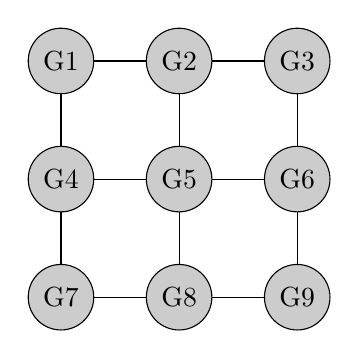
\begin{tikzpicture}[darkstyle/.style={circle,draw,fill=gray!40,minimum size=5}]
\foreach \y in {0,1,2}
 \foreach \x in {0,1,2}
{\pgfmathtruncatemacro{\label}{\x-3*\y+7}
\node[darkstyle](\x\y) at (1.5*\x,1.5*\y){G\label};
}
 \foreach \x in {0,1,2}
    \foreach \y [count=\yi] in {0,1}  
      \draw (\x\y)--(\x\yi) (\y\x)--(\yi\x) ;

\end{tikzpicture}

\caption{Actual arrangement}
\label{fig:symm}
}


\ffigbox{
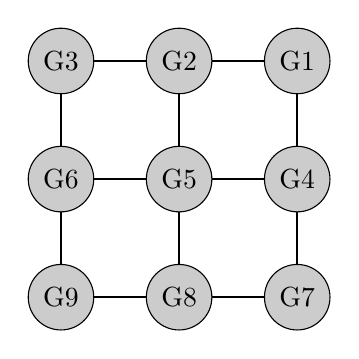
\begin{tikzpicture}[darkstyle/.style={circle,draw,fill=gray!40,minimum size=5}]

\draw[step = 1.5,thick ] (7.4,0) grid (10.5,3);
\node[circle,draw=black,fill=white!80!black,minimum size=5] (7) at (7.5,0) {G9};
\node[circle,draw=black,fill=white!80!black,minimum size=5] (4) at (7.5,1.5) {G6};
\node[circle,draw=black,fill=white!80!black,minimum size=5] (1) at (7.5,3) {G3};

\node[circle,draw=black,fill=white!80!black,minimum size=5] (8) at (9,0) {G8};
\node[circle,draw=black,fill=white!80!black,minimum size=5] (5) at (9,1.5) {G5};
\node[circle,draw=black,fill=white!80!black,minimum size=5] (2) at (9,3) {G2};

\node[circle,draw=black,fill=white!80!black,minimum size=5] (9) at (10.5,0) {G7};
\node[circle,draw=black,fill=white!80!black,minimum size=5] (3) at (10.5,1.5) {G4};
\node[circle,draw=black,fill=white!80!black,minimum size=5] (6) at (10.5,3) {G1};
%\draw [<->,red] (3.east) to [out=60,in=60] (6.east);

\end{tikzpicture}

\caption{Sensors arrangement rotationally symmetric to the actual arrangement }
\label{fig:rotationalSymm}
}
\centering

\end{floatrow}
\end{figure}


\subsection{Special case when the grid is $n \times 2$ or $2 \times n$}
Consider a $2 \times n$ sensor grid with diagonally opposite nodes connected as shown in the Figure \ref{fig:ntime2}. These grid structure posses a special case of symmetry. As shown in the  Figure \ref{fig:ntime2Sym} nodes 1 and 2 are interchanged; it is as if the whole structure was rotated with  edge (1,2) fixed. The diagonally opposite edges (1,3) in Figure \ref{fig:ntime2} becomes non diagonal edges in the Figure \ref{fig:ntime2Sym}. To overcome this error we use a \textit{Weighted Grid Adjacency Matrix (WGAM)} instead of a binary grid adjacency matrix. We compute $(WGAM)$ first by taking the reciprocal of the distance between the nodes which has an edge between them in the $GAM$ and then normalizing it by multiplying with the least distance ($d_{min}$) that exists between two nodes in the entire grid. All the values in the $WGAM$  lie between 0 and 1. A value close to 1 signifies that the 2 vertices are close to each other and a value close to 0 signifies that the 2 vertices are far away from each other.
\begin{equation}
WGAM_{i,j} = 
\begin{cases}
\dfrac{d_{min}}{d_{i,j}}, &\text{ if } GAM_{i,j} = 1\\
0, & \text{otherwise}\\
\end{cases}
\end{equation}

We use $WGAM$ instead of $GAM$ to compute $GCS$ in equation \ref{eq:gridCorrelationSum}. The reasoning behind the use of $WGAM$ matrix instead of the $GAM$ is that we hypothesize that the correlation values for the sensor which are closer are higher than the one compared to sensors which are further apart. By assigning weights to the edges in this manner, more importance is given to the edges between the sensors that are close to the each other. Doing so the sensors which are close by contribute  more to the $GCS$ . 
Now if we consider arrangement as shown in the Figure \ref{fig:ntime2} and \ref{fig:ntime2Sym} though their $GCS$ remain the same, when computed using $GAM$, $GCS$ won't remain the same when $GAM$ is substituted by $WGAM$. The contribution of the correlation between the sensors placed on the nondiagonal edges is more compared to the contribution made by the diagonal edges to $GCS$. Therefore if we place the non-diagonally located sensors on the diagonals of the grid, $GCS$ decreases. Thus by using a \textit{Weighted Grid Adjacency Matrix} we are able to obtain the mapping of the sensors onto the grid upto rotational symmetry.

\begin{figure}
\begin{floatrow}
\ffigbox{

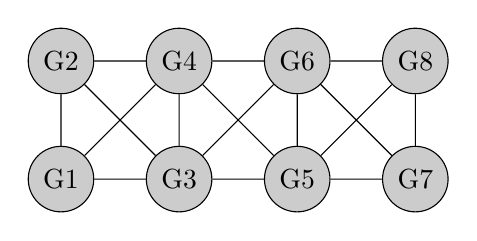
\begin{tikzpicture}

\node[circle,draw=black,fill=white!80!black,minimum size=5] (1) at (0,0) {G1};
\node[circle,draw=black,fill=white!80!black,minimum size=5] (3) at (1.5,0) {G3};
\node[circle,draw=black,fill=white!80!black,minimum size=5] (5) at (3,0) {G5};
\node[circle,draw=black,fill=white!80!black,minimum size=5] (7) at (4.5,0) {G7};
\node[circle,draw=black,fill=white!80!black,minimum size=5] (2) at (0,1.5) {G2};
\node[circle,draw=black,fill=white!80!black,minimum size=5] (4) at (1.5,1.5) {G4};
\node[circle,draw=black,fill=white!80!black,minimum size=5] (6) at (3,1.5) {G6};
\node[circle,draw=black,fill=white!80!black,minimum size=5] (8) at (4.5,1.5) {G8};
\draw (1)--(2) (1)--(3) (1)--(4) (2)--(3) (3)--(4) (4)--(6)   (2)--(4)  (4)--(5) (3)--(6) (3)--(5) (5)--(6) (6)--(7) (5)--(8) (5)--(7) (7)--(8) (8)--(6);
\end{tikzpicture}
\caption{Actual arrangement of $2 \times 4$ grid.}
\label{fig:ntime2}
}

\ffigbox{
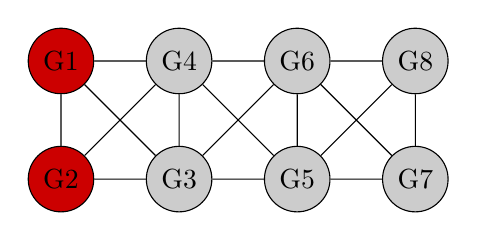
\begin{tikzpicture}
\node[circle,draw=black,fill=red!80!black,minimum size=5] (2) at (0,0) {G2};
\node[circle,draw=black,fill=white!80!black,minimum size=5] (3) at (1.5,0) {G3};
\node[circle,draw=black,fill=white!80!black,minimum size=5] (5) at (3,0) {G5};
\node[circle,draw=black,fill=white!80!black,minimum size=5] (7) at (4.5,0) {G7};
\node[circle,draw=black,fill=red!80!black,minimum size=5] (1) at (0,1.5) {G1};
\node[circle,draw=black,fill=white!80!black,minimum size=5] (4) at (1.5,1.5) {G4};
\node[circle,draw=black,fill=white!80!black,minimum size=5] (6) at (3,1.5) {G6};
\node[circle,draw=black,fill=white!80!black,minimum size=5] (8) at (4.5,1.5) {G8};
\draw (1)--(2) (1)--(3) (1)--(4) (2)--(3) (3)--(4) (4)--(6)   (2)--(4)  (4)--(5) (3)--(6) (3)--(5) (5)--(6) (6)--(7) (5)--(8) (5)--(7) (7)--(8) (8)--(6);


\end{tikzpicture}
\caption{Incorrect arrangement of $2 \times 4$ grid with the same $GCS$ values.}
\label{fig:ntime2Sym}
}
\centering
\end{floatrow}
\end{figure}


\section{Summary}
In this chapter, we described a method to locate the sensor on the grid by using the data from the sensors and grid vertices information up-to rotational symmetry. We show how graph matching technique can be used to obtain the possible mappings between the sensors and grid vertices. Using the correlation values between the sensors we determine a criteria that helps to choose the true arrangement out of the obtained possible arrangements. We also resolve the issue that arises when the grid is either a $n \times 2$ or $2 \times n$ grid using a weighted grid adjacency matrix. Figure \ref{fig:Summary} gives the summary of steps involved in the form of a flowchart. 

\begin{figure}
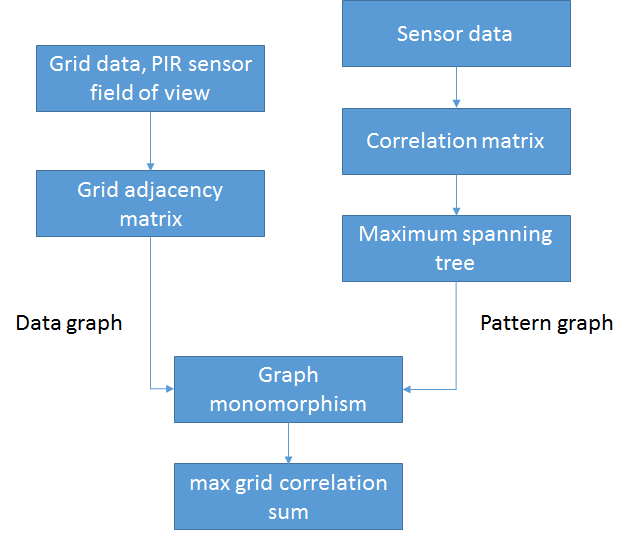
\includegraphics[scale=0.49]{./pics/methodSummary.png}
\caption{Flowchart summarizing the developed method.}
\label{fig:Summary}
\centering
\end{figure}



 






 


